\section*{Tests and metrics}

...

\begin{figure}[h!t]
    \centering
    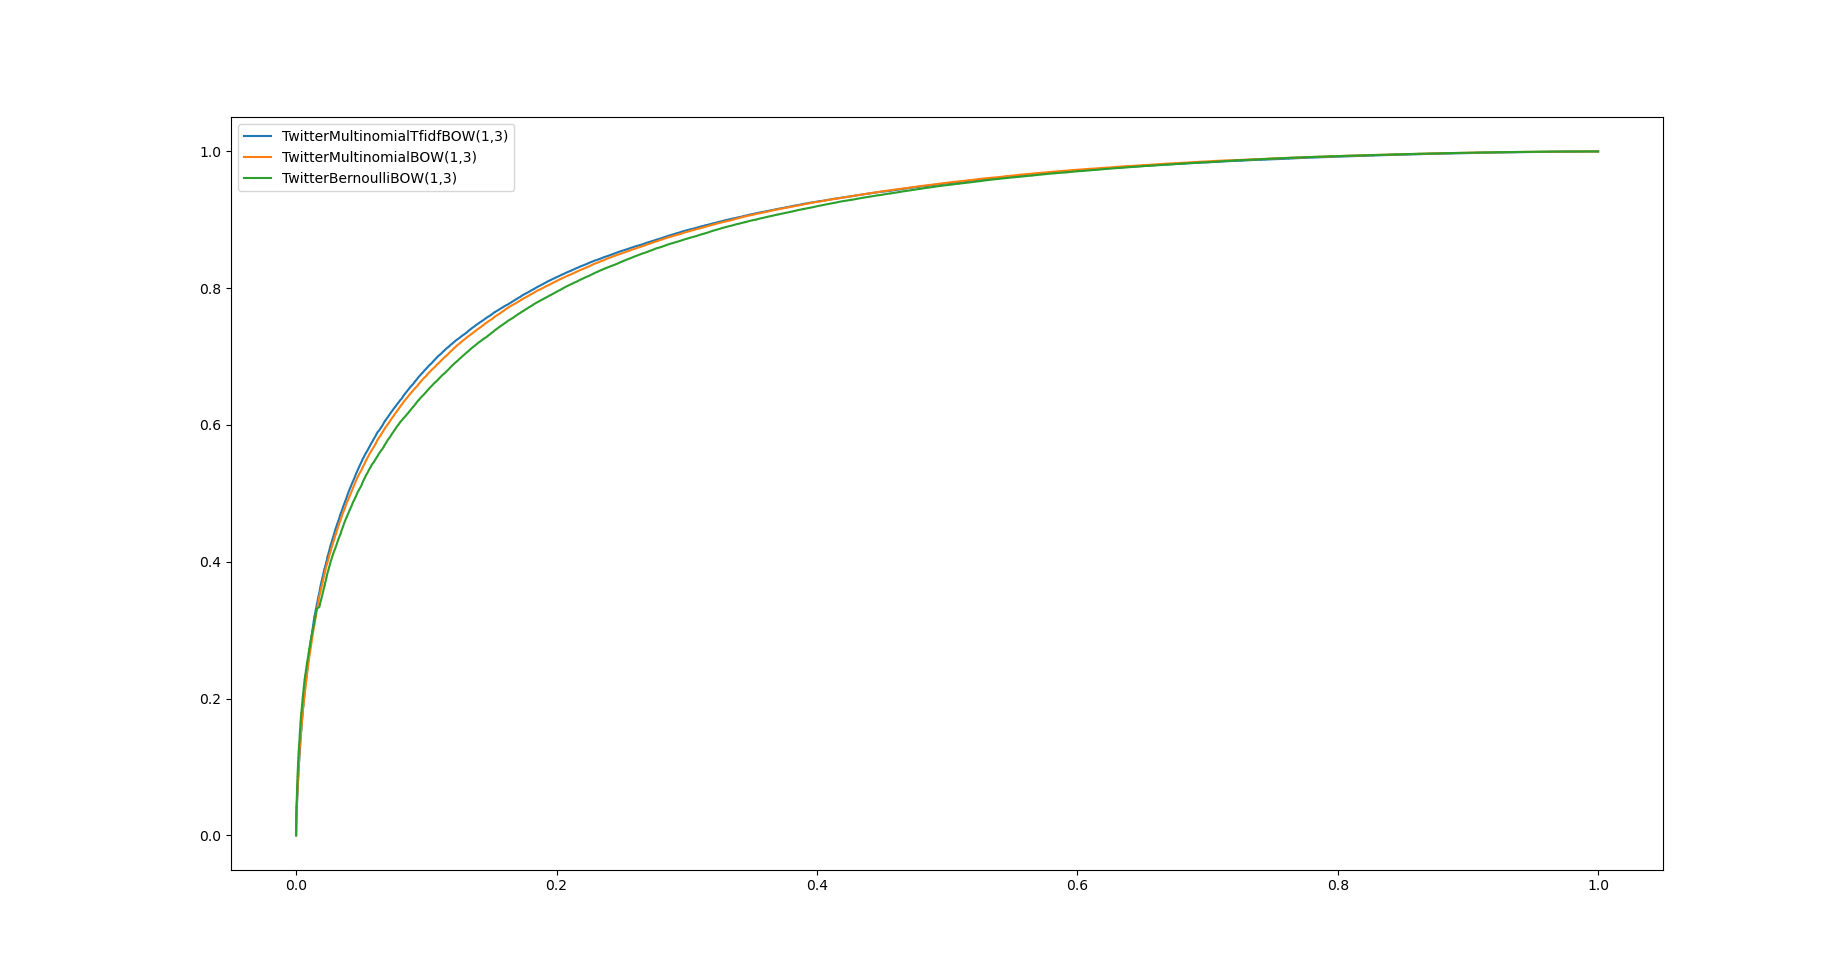
\includegraphics[scale=0.25]{../experiments/plots/TwitterBOWTfidf}
    \caption{ROC curve for the Na\"ive Bayes approach with tf-idf.}
    \label{fig:ROCNB}        
\end{figure}

\begin{figure}[h!t]
    \centering
    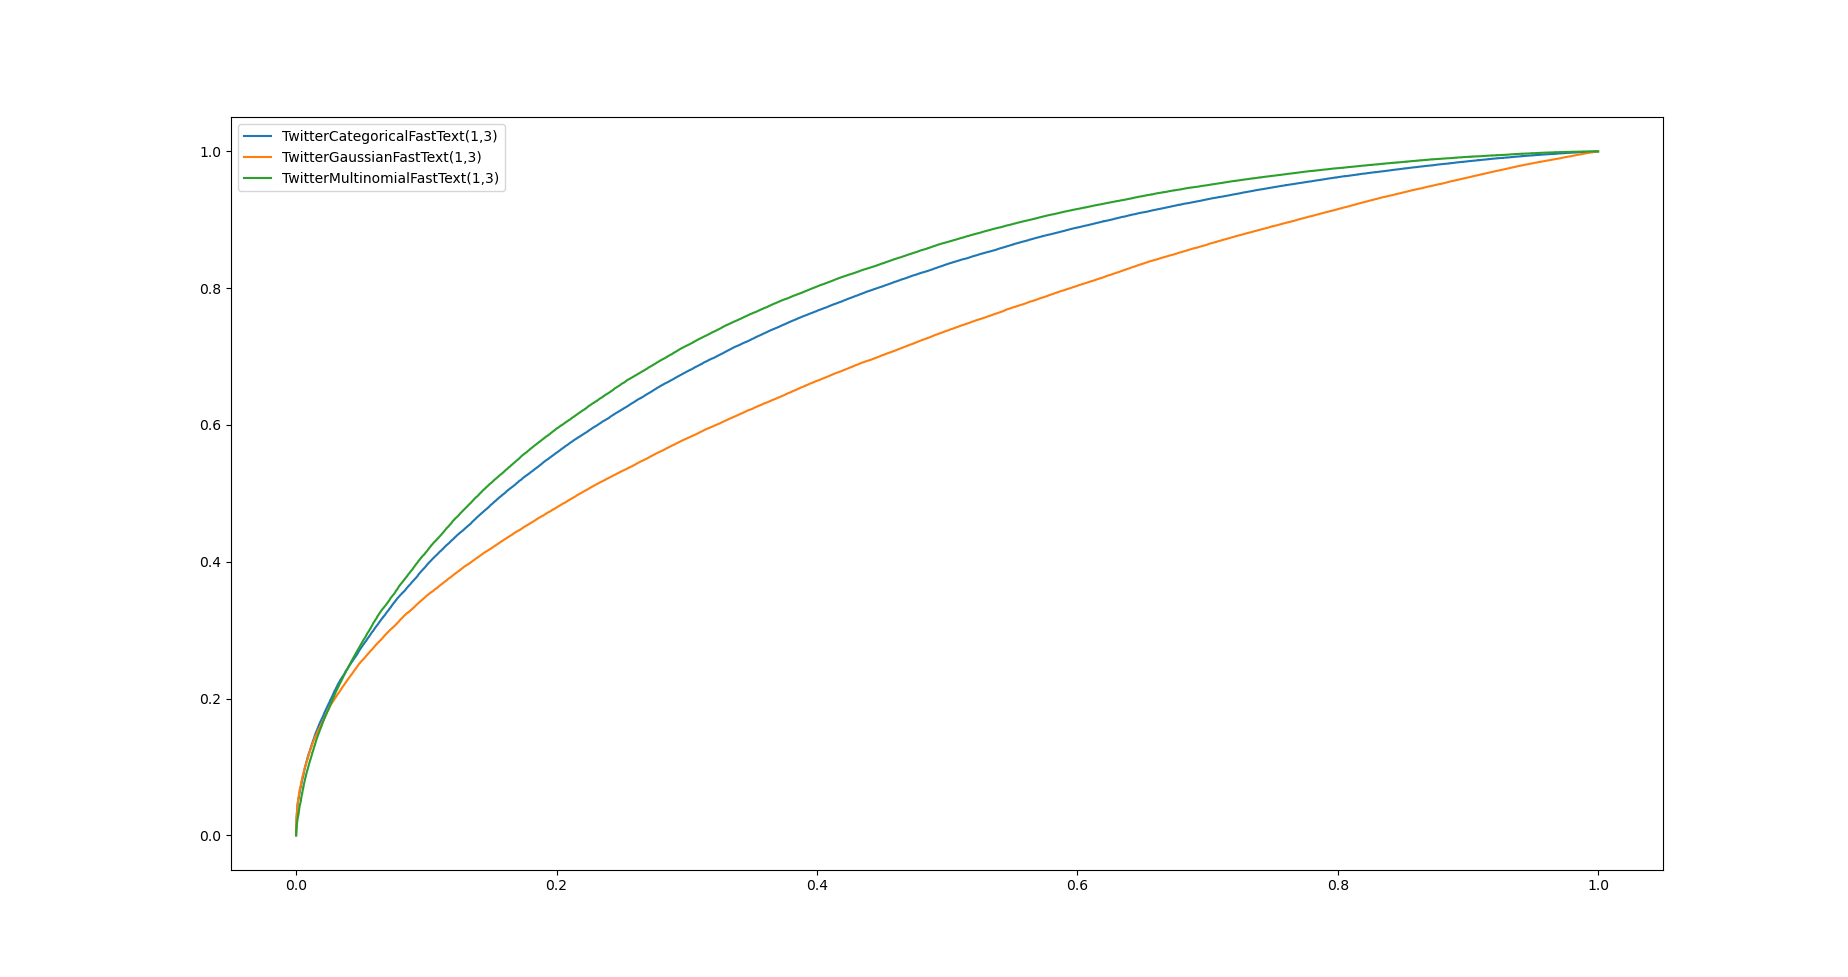
\includegraphics[scale=0.25]{../experiments/plots/TwitterFastText}
    \caption{ROC curve for the FastText embedding.}
    \label{fig:ROCFT}
\end{figure}

\subsection*{Kaggle notebooks}

\subsection*{Further tests}
We trained our model with a dataset and tested it against a different one, to this aim were used am IMDb dataset of cinematographic reviews ~\cite{data:imdb} and a Reddit one about various NFL games ~\cite{data:reddit}, results for the Bag-Of-Words Na\"ive Bayes (1,3)-gram model can be seen in figures \ref{fig:TwitterImdb} and \ref{fig:TwitterReddit}.

\begin{figure}[h!t]
    \centering
    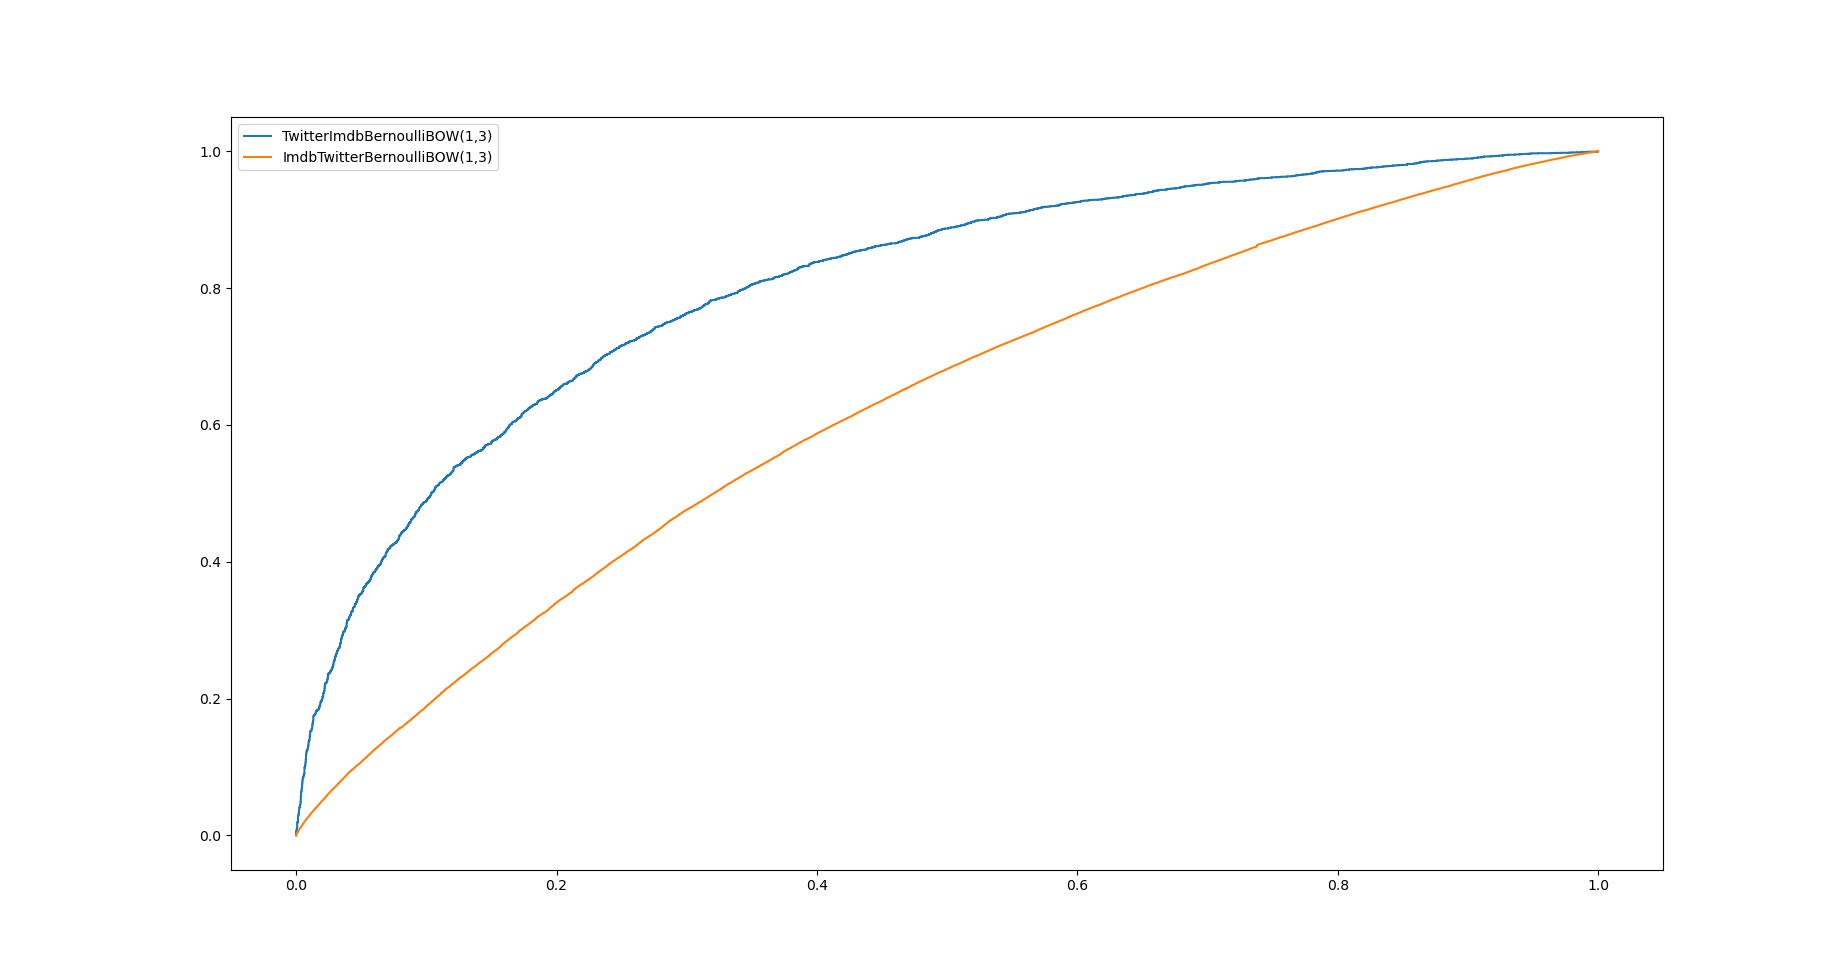
\includegraphics[scale=0.25]{../experiments/plots/ImdbTwitter}
    \caption{Comparison between Imdb-Twitter and Twitter-Imdb.}
    \label{fig:TwitterImdb}        
\end{figure}

\begin{figure}[h!t]
    \centering
    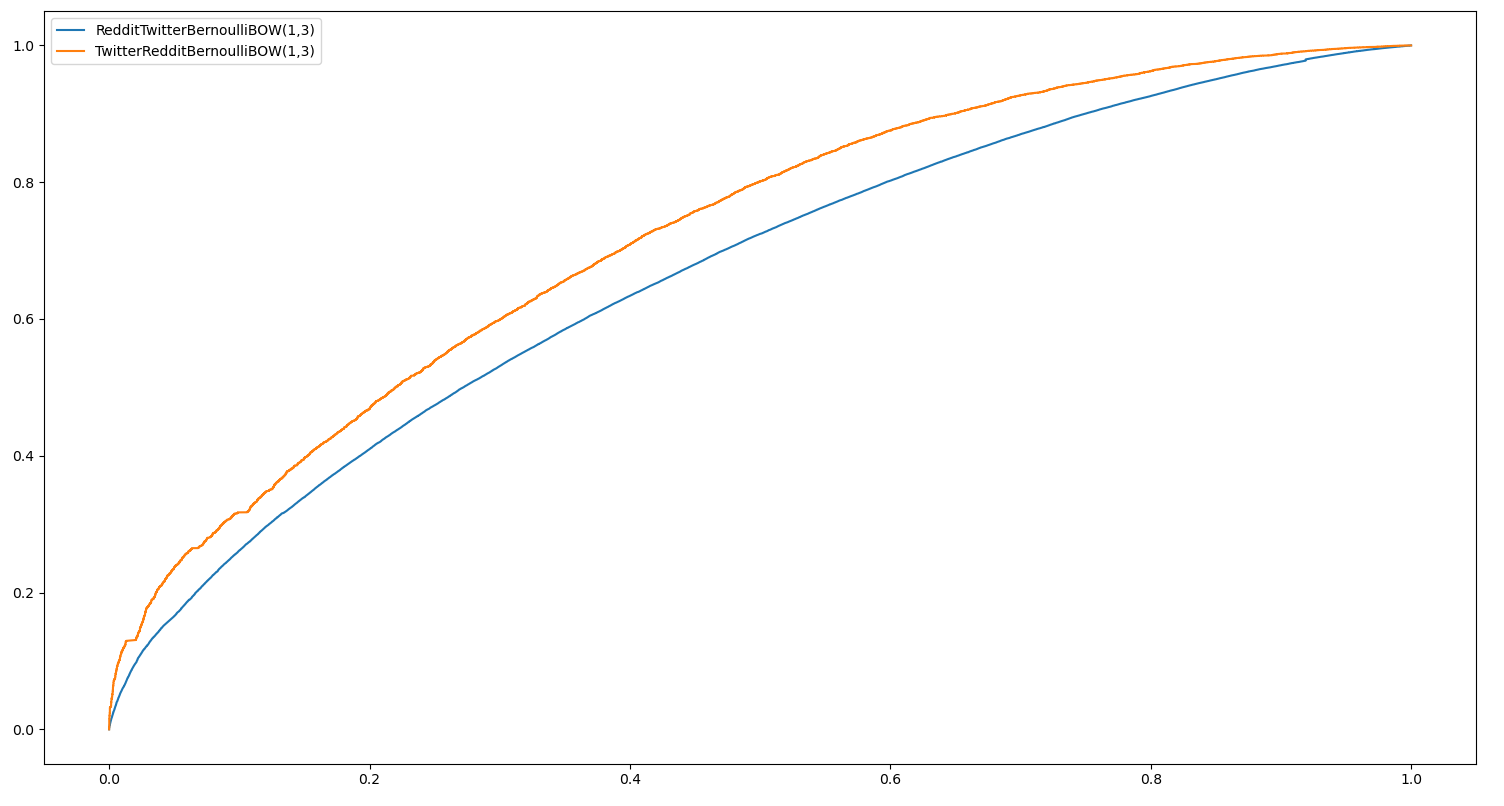
\includegraphics[scale=0.25]{../experiments/plots/RedditTwitter}
    \caption{Comparison betwen Reddit-Twitter and Twitter-Reddit.}
    \label{fig:TwitterReddit}
\end{figure}

This is something usually not done since different datasets will have different distributions hence we expect bad results, strangely enough training our model with the Twitter dataset and testing it with the IMDb one gives rather good metrics that can be seen in table \ref{tab:versus_metrics}, is exposed only the comparision betwen Twitter and IMDb since results are more interesting. 
This could happen since Twitter's dataset has a very large number of examples, other datasets other than being smaller are also very specific: the Reddit one is only about a specific set of american football games and the IMDb one is about cinematographic reviews, reasonably in this case lexicon is also more specific. 
Sentiment140 on the other hand covers a larger class of human language and is less prone to be biased.

\begin{table}[h!t]
    \centering
    \caption{Comparing metrics for some train test combinations.}
    \label{tab:versus_metrics}
    \begin{tabular}{c|ccc}
        \hline
        Train-Test & Accuracy & F1 & AUROC \\
        \hline 
        Twitter-IMDb & 0.732 & 0.723 & 0.806 \\ 
        IMDb-IMDb & 0.891 & 0.887 & 0.963 \\ 
        IMDb-Twitter & 0.550 & 0.330 & 0.625 \\ 
        Twitter-Twitter & 0.797 & 0.800 & 0.880 \\ 
        \hline
    \end{tabular}
\end{table}
